\documentclass[10pt]{beamer}

\usetheme{m}

\usepackage{booktabs}
\usepackage[scale=2]{ccicons}

\usepackage{multicol}

\usepackage{pgfplots}
\usepgfplotslibrary{dateplot}

\usepackage{upgreek}

 
\newtheorem{examplenegative}{exampleblock}
\newenvironment<>{examplenegative}[1]{%
  \setbeamercolor{block title example}{fg=red}%
  \begin{exampleblock}#2{#1}}{\end{exampleblock}}


\setbeamercovered{invisible}

%Notes on laptop but not on presentation
%\usepackage{pgfpages}
%\setbeameroption{show notes}
%\setbeameroption{show notes on second screen=right}
%\setbeameroption{show notes on second screen}

\usepackage[]{algorithm2e}
\makeatletter
\usepackage{color}
\definecolor{editorLightGray}{cmyk}{0.05, 0.05, 0.05, 0.1}
\definecolor{editorGray}{cmyk}{0.6, 0.55, 0.55, 0.2}
\definecolor{editorPurple}{cmyk}{0.5, 1, 0, 0}
\definecolor{editorWhite}{cmyk}{0, 0, 0, 0}
\definecolor{editorBlack}{cmyk}{1, 1, 1, 1}
\definecolor{editorOrange}{cmyk}{0, 0.8, 1, 0}
\definecolor{editorBlue}{cmyk}{1, 0.6, 0, 0}
\definecolor{editorPink}{cmyk}{0, 1, 0, 0}
\usepackage{upquote}
\usepackage{listings}
% CSS
\lstdefinelanguage{CSS}{
  keywords={color,background-image:,margin,padding,font,weight,display,position,top,left,right,bottom,list,style,border,size,space,min,width, transition:, transform:, transition-property, transition-duration, transition-timing-function, background:, color:, background-color:}, 
  sensitive=true,
  morecomment=[l]{//},
  morecomment=[s]{/*}{*/},
  morestring=[b]',
  morestring=[b]",
  alsoletter={:},
  alsodigit={-}
}

% JavaScript
\lstdefinelanguage{JavaScript}{
  morekeywords={typeof, new, true, false, catch, function, return, null, catch, switch, var, if, in, while, do, else, case, break},
  morecomment=[s]{/*}{*/},
  morecomment=[l]//,
  morestring=[b]",
  morestring=[b]'
}

\lstdefinelanguage{HTML5}{
  language=html,
  sensitive=true,   
  alsoletter={<>=-+},   
  morecomment=[s]{<!-}{-->},
  tag=[s],
  otherkeywords={
  % General
  % >,
  % Standard tags
    <!DOCTYPE,
  </html, <html, <head, <title, </title, <style, </style, <link, </head, <meta, />,
    % body
    </body, <body,
    % Divs
    </div, <div, </div>, 
    % Paragraphs
    </p, <p, </p>,
    % scripts
    </script, <script,
  % More tags...
  <canvas, /canvas>, <svg, <rect, <animateTransform, </rect>, </svg>, <video, <source, <iframe, </iframe>, </video>, <image, </image>
  },
  ndkeywords={=,
  % General
  +=,
  % HTML attributes
   charset=, src=, id=, width=, height=, style=, type=, rel=, href=,
  % SVG attributes
  fill=, attributeName=, begin=, dur=, from=, to=, poster=, controls=, x=, y=, repeatCount=, xlink:href=,
  % CSS properties
  margin:, padding:, background-image:, border:, top:, left:, position:, width:, height:,
    % CSS3 properties
  transform:, -moz-transform:, -webkit-transform:,
  animation:, -webkit-animation:,
  transition:,  transition-duration:, transition-property:, transition-timing-function:,
  },
}



\makeatother


\title{App-udvikling}
\subtitle{6. Lektion}
\date{\today}
\author{Sune Sylvest Nilausen}
%\institute{Institute or miscellaneous information}
% \titlegraphic{\hfill\includegraphics[height=1.5cm]{logo/logo}}

\begin{document}
%\setbeamertemplate{caption}{\raggedright\insertcaption\par}

\maketitle

\begin{frame}
  \frametitle{Indholdsfortegnelse}
  \setbeamertemplate{section in toc}[sections numbered]
  \tableofcontents[hideallsubsections]
\end{frame}
%Forhenværende lektioner gik ud på at lære de første trin i at designe et produkt.
%Altså at designe et app.

\section{Opsummering fra sidst}

\begin{frame}[fragile]
 \frametitle{HTML Kode}

\lstset{
  language=html,
  tagstyle=\color{editorBlue},
  basicstyle={\small\ttfamily},
  identifierstyle=\color{editorOrange},
  keywordstyle=\color{editorPink},
  commentstyle=\color{editorGray},
  stringstyle=\color{editorPurple}
}
\begin{lstlisting}
<!DOCTYPE html>
<html>
  <body>
    <!-- Kommentar -->
    <div id="box">
      <p>Hello World</p>
      <h1>Overskrift type 1</h1>
      <h2>Overskrift type 2</h2>
      <img src="html5.png" width="250px" height="250px">
    </div>
    <div>Test</div>
  </body>
</html>
\end{lstlisting}
\end{frame}

\begin{frame}{HTML Syntax}
		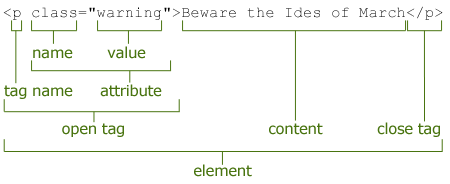
\includegraphics[width=\linewidth]{img/html-syntax.png}
\end{frame}


\begin{frame}[fragile]
 \frametitle{CSS Kode}

\lstset{
  language=HTML5,
  alsolanguage=CSS,
  tagstyle=\color{editorBlue},
  basicstyle={\small\ttfamily},
  identifierstyle=\color{editorOrange},
  keywordstyle=\color{editorPink},
  commentstyle=\color{editorGray},
  stringstyle=\color{editorPurple}
}
\begin{lstlisting}
h1 { color: white;
background: orange;
border: 1px solid black;
}
body {background-color: white;
color: black;
border: 12px solid;
}
/* Kommentar */
\end{lstlisting}
\end{frame}

\begin{frame}{CSS Syntax}
		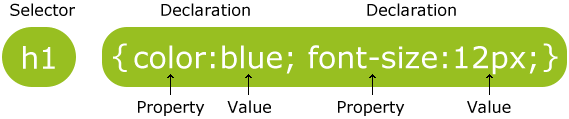
\includegraphics[width=\linewidth]{img/css-syntax.png}
\end{frame}



\section{Chrome Dev Editor!}
\begin{frame}{Install it!}
	install it!
\end{frame}


\section{HTML App}
\begin{frame}{Hurtigt interface}
	Sådan bruger du bootstrap, polymer, andre ting til hurtigt at lave interface.
\end{frame}

\begin{frame}{Opgave:}
	1. Lav nogle opgaver \\
	2. Lav interface til dit projekt.
\end{frame}

\section{CSS App}
\begin{frame}{Opgave:}
	1. Lav nogle opgaver \\
	2. Lav styling til dit projekt.
\end{frame}

\section{Javascript App}
\begin{frame}{Opgave:}
	1. Lav nogle opgaver \\
	2. Lav noget programstyring til dit projekt.
\end{frame}

\section{App med det hele}
\begin{frame}{Opgave:}
	1. Færdiggør dit projekt
\end{frame}

\plain{
\url{http://io2014codelabs.appspot.com/static/codelabs/chrome-apps/#1}
 }

\plain{
\url{http://io2014codelabs.appspot.com/static/codelabs/polymer-build-maps/#1}
}
 

\end{document}
